\documentclass{article}
\usepackage[utf8]{inputenc}

\title{Main Locations Extraction in Literature}
\author{Ohad Edelstein (ID 039065313), Nitzan Katz (ID 318446929)}
\date{Submitted as final project report for NLP, IDC, 2020}

\usepackage{natbib}
\usepackage{graphicx}
\usepackage{hyperref}
\usepackage{wrapfig}
\usepackage{xcolor,colortbl}

\begin{document}

\maketitle

\section{Introduction}

The purpose of this project is to extract the locations related to main characters in books. This may contribute to a bigger task of making a site-seeing route based on the route of main characters in archaeology books. The project includes POS (part of speech) tagging and NER (name entity recognition) in books, characters relational graph based on sentiment analysis and characters-locations co-occurrences graph. We mostly rely on commonly used models for solving this issue rather than inventing new models for the specific tasks.

\subsection{Related Works}
The main work we referred to is a github project\cite{hzjken2019char} in which the author extracted the characters out of the harry potter series, and made two types of relational graph between them. One graph is made based on co-occurrences of the characters in the books, and the other was made using sentiment analysis over the sentences more than one character was involved in order to determine the nature of the relationship (whether it's good or bad, and how strong it is). We thought about taking this concept and checking if the characters with the most relations to other characters can be classified as the main characters, and furthermore use the co-occurrences of those characters to locations to determine the main locations from the book.

\pagebreak
\section{Solution}
\subsection{General approach}
We started the project with a wide internet research on character detection in books. The initial idea was to find an approach for extracting the interesting characters in books and try to convert it to locations instead.\newline
Shortly into the reading we found the main project we relied on, with the general idea of making a relation graph between the characters in a book to find its main characters. We wanted to try and see if the same technique can be used to find the main locations of the book based on their connections with the main characters.\newline
The project focused only on the Harry Potter series, which is nice for a proof-of-concept for the characters idea, but since most of the names and locations are made up, we soon found out that locations identification isn't that straight forward. However, our main goal is archaeology books with real places, so we decided to keep going with the idea and try it on other books with stories happening in real locations (Patriot Games by Clancy Tom).

\subsection{Design}
The original project is made out of 4 parts in general: Data Preparation for the processing parts, NER for retrieving the characters and locations, character importance to filter out the non-interesting characters, co-occurrence matrix to find relations between characters and places.
\subsubsection{Data Preparation}
Before the processing of the data itself we need to prepare the data to work on. That involves both getting the novels, which we got from the project Gutenberg\cite{projectgutenberg}, and defining a list of commonly used words in English in order to filter out words from the NER process that got mis-tagged. We just used the same definition as the one used in the original project.
\subsubsection{Name Entity Recognition}
For the NER task we used the SpaCy NER classifiers\cite{spacy}, which are pre-trained classifiers that are commonly used in such projects (Both model used trained over the OntoNotes 5\cite{ontonotes} with one model using GloVe vectors). At this part, we go over each sentence from the book and extract the names and the locations. At this part, we also split the full names into the words, that's because sometimes a character is being referred by its full name, and sometimes by its first/last name instead. After that names that are in the common English words list are removed, and names that appear less than a certain threshold are removed (to filter outliers and very uncommon characters).
\subsubsection{Character Importance}
The character importance is determined mostly by the appearances of that character in the book. With the same concept, we filter the important places by the places that appeared the most in the book. With a smaller set of names and locations the calculation and visualization of the relations graphs becomes possible in relatively small amount of time.
\subsubsection{Co-occurrence Matrix}
The co-occurrence matrix is calculated solely on the appearance of two characters (and character and a location) in the same sentence, since this is the method in which we go over the book. The method is simple, we first create a binary indication for each sentence and word if the word appeared in the sentence, then we just multiply the matrix by itself to find the cross-appeared words. After that, we triangularize the matrix since it's symmetrical, and remove the diagonal values because we don't mind words that appear with themselves. The process is described in figure 1.
\begin{figure}[h]
  \centering
  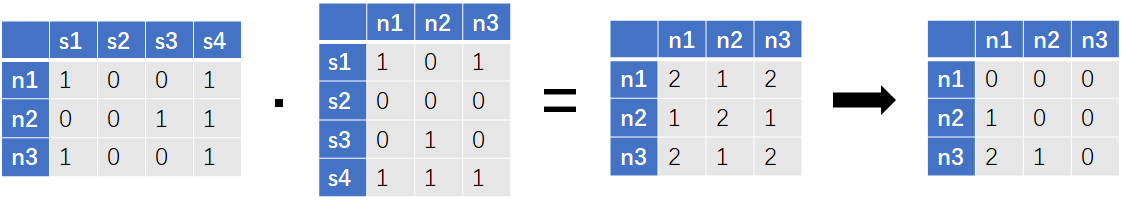
\includegraphics[width=10cm]{co-occurences_defintion.png}
  \caption{Co-occurrence Matrix Build}
  \label{fig1}
\end{figure}
After the matrix is created, we can easily turn it into a graph, normalizing the color of the edge of each connection by the amount of relations related to the others in the matrix. First sanity reasons, we also calculated the sentiment matrix between the characters. Both because it is interesting on its own in showing the relations between the main characters of the book, but also to see that the results shown in the original project are valid.

\section{Experimental results}
At first, we recreated the results shown in the project. For that we cloned the project and mostly ran it as it is. We also downloaded the relevant Harry Potter books to see if it works. The results were identical to what shown in the project, so we kept with the idea.

Now, we needed to extract the locations out of the book. For that, we looked into the SpaCy models, and saw the relevant labeling for locations. The label "GPE", "LOC" and "FAC" are our indication of places in the book. The locations we found in Harry Potter: Sorcerer's Stone were pretty interesting. The list we got is: 'firenze', 'london', 'flint', 'romania', 'privet drive', 'uncle vernon', 'smelting stick'. Which contains both real locations, like firenze, and london, but also misfits from the algorithm, like privet drive or uncle vernon. However, as seen in figure 2, only the real locations receive a serious enough relation to be noticeable in the graph itself (There are connections between some of the other characters and locations, it's too low to be seen as the strength of the color is determined by the amount of co-occurrences). We also had some issues with names there were mis-interpreted as locations, which we removed later if they were labeled as both names and locations (we decided to include them as just names).
\begin{figure}[h]
  \centering
  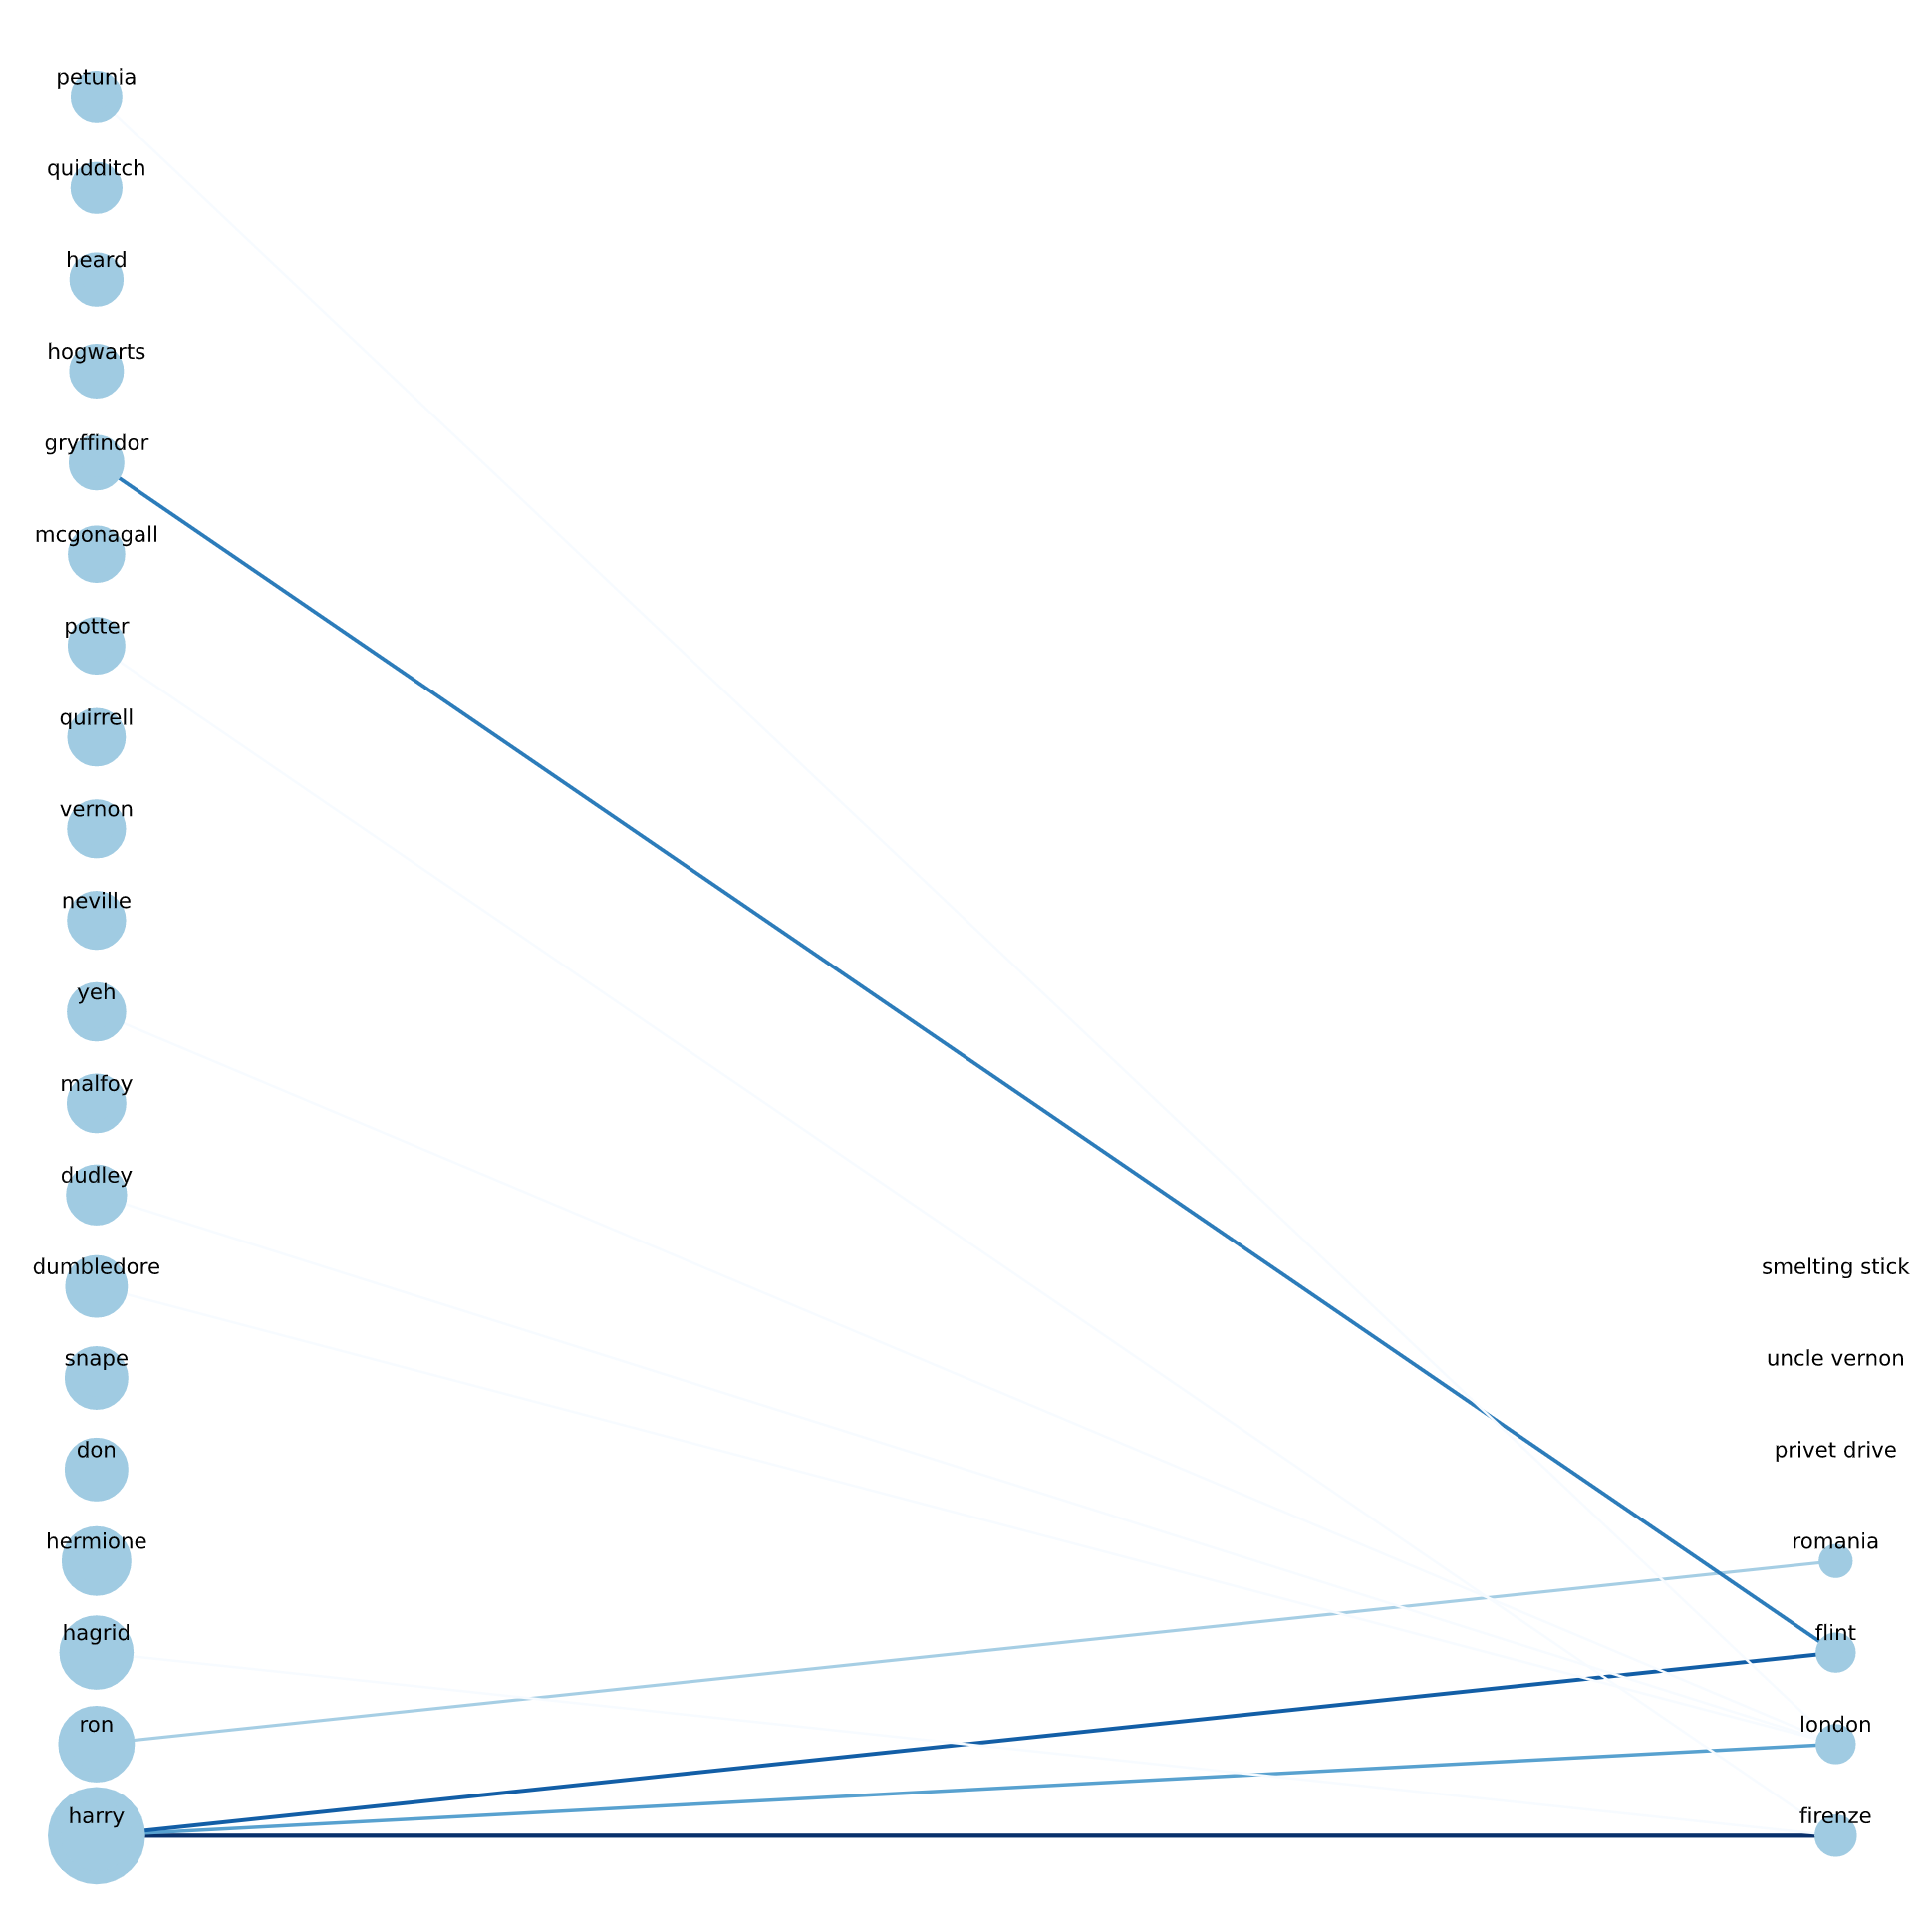
\includegraphics[width=10cm]{Harry Potter 1 - Sorcerer's Stone locations graph.png}
  \caption{Harry Potter: Sorcerer's Stone Locations Graph}
  \label{fig2}
\end{figure}

To calculate the relations between the locations and the characters we mostly combined the names and the locations after the most common names and locations were filtered and used the same matrix creation as before. Then we only use the results regarding the relations between the parts of the names with the parts of the locations.

At this point we still didn't have the graph shown here, there were still adjustments needed to the graph painting algorithm, as a circle-like cross-connections isn't as intuitive for showing the connections between two groups.

Also, the running time of a notebook in this way took around 15 minutes to run. This was mostly because the split to separate parts that go over the book each time and calculate different things made a big overhead. The extractions of locations, names and affinity were combined and improved the processing time significantly.

After we had these results on the Harry Potter book, we wanted to see on a non-fiction world based book to see what results we will receive. We chose Clancy Tom's book "Patriot Games" and created a generic notebook that does the whole process given the path to the book's file.

Here it's also interesting to see the co-occurrence graph and see the relations between the characters, since so far it was only tested on Harry Potter. From the relations graph in figure 3 we can see the main character Jack Ryan as the characters with most strong connections (Jack), also with Cathy which is Jack's wife and also a main character and Sally, his daughter. All three of them have the last name Ryan which is also shows as main in here which makes sense.
\begin{figure}[h]
  \centering
  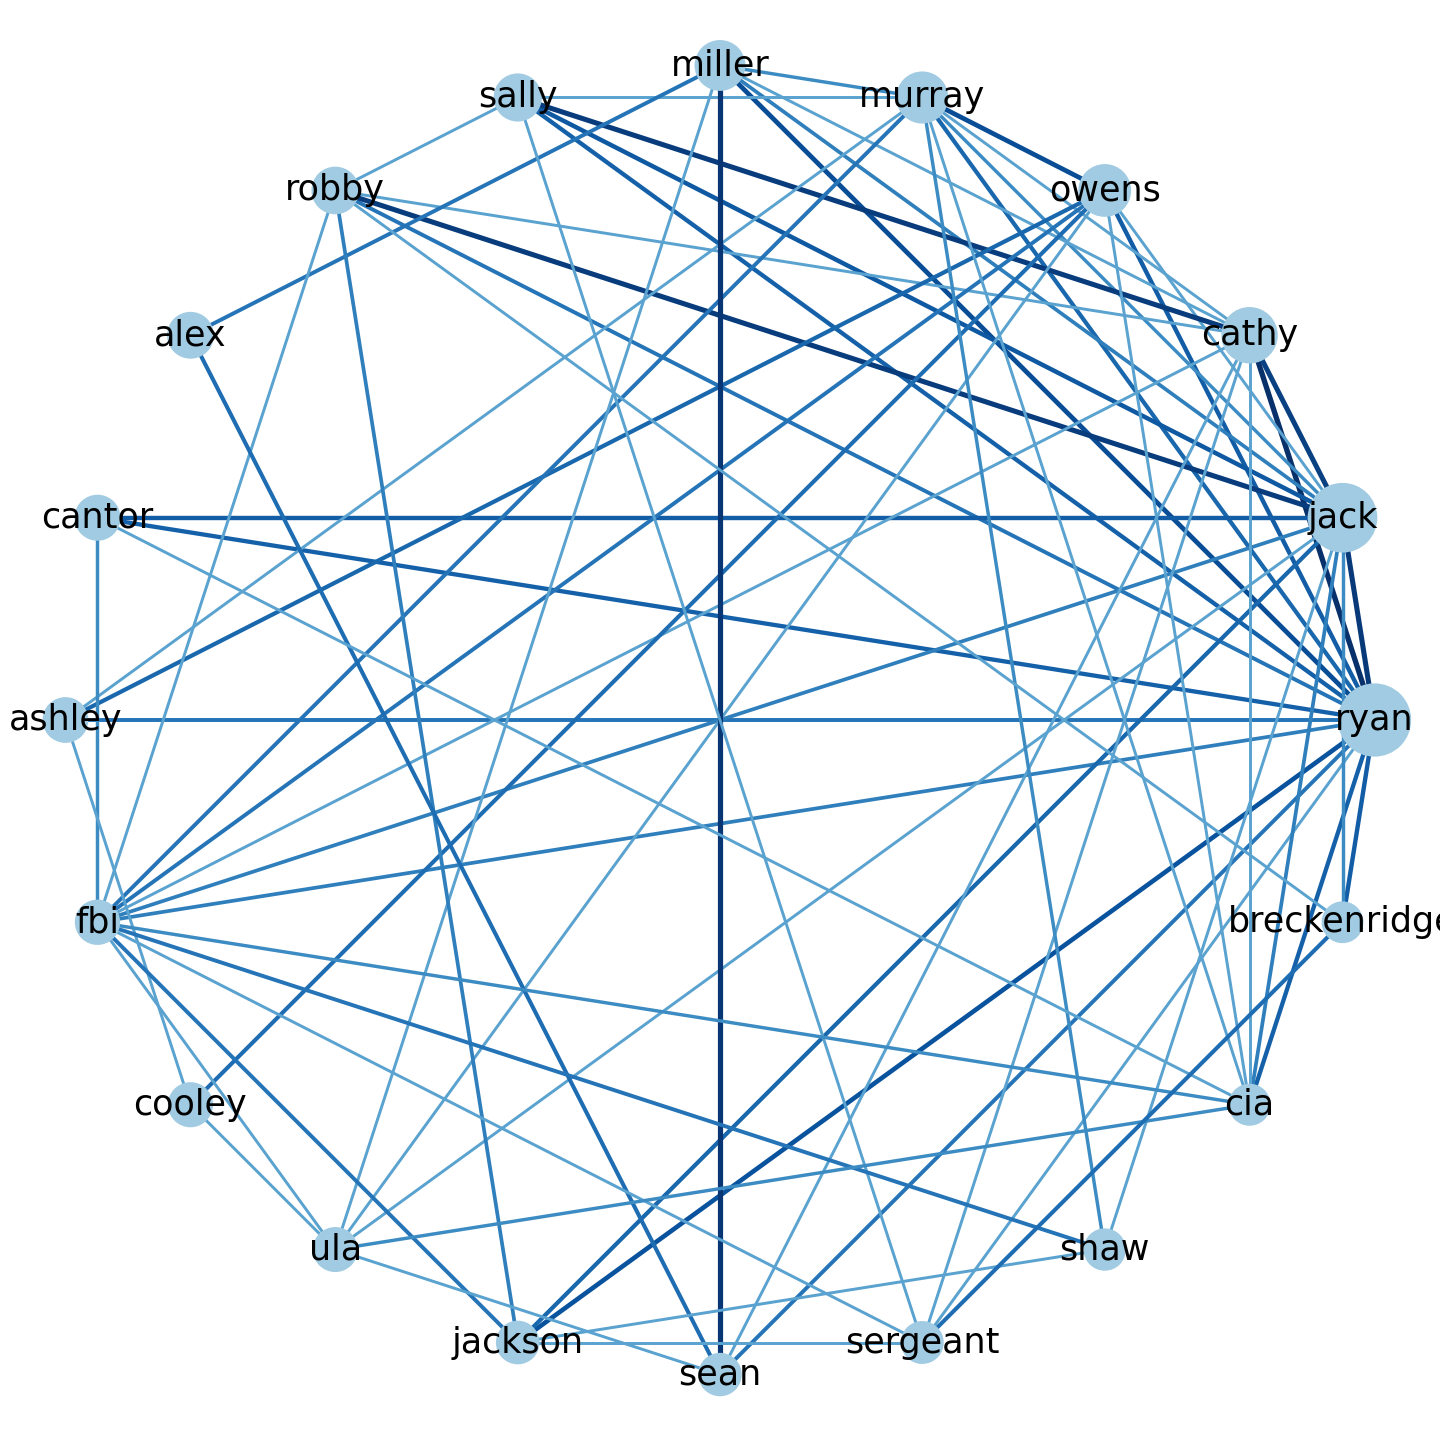
\includegraphics[width=10cm]{Tom Clancy co-occurrence graph.png}
  \caption{Clancy Tom Patriot Game Co-occurrence Graph}
  \label{fig3}
\end{figure}

Since the relations graph makes sense, we continued for the characters-locations relations graph. The results are pretty interesting (figure 4) the main locations are London, America, Baltimore, Annapolis and Washington which are indeed related to the plot of the story. Notice that there's a strong connection between Sergeant and Highland, when we're not familiar in detail with the book we can't make sense of a location name Highland on it's own. It might be another main location, and it might be an outlier.

\begin{figure}[h]
  \centering
  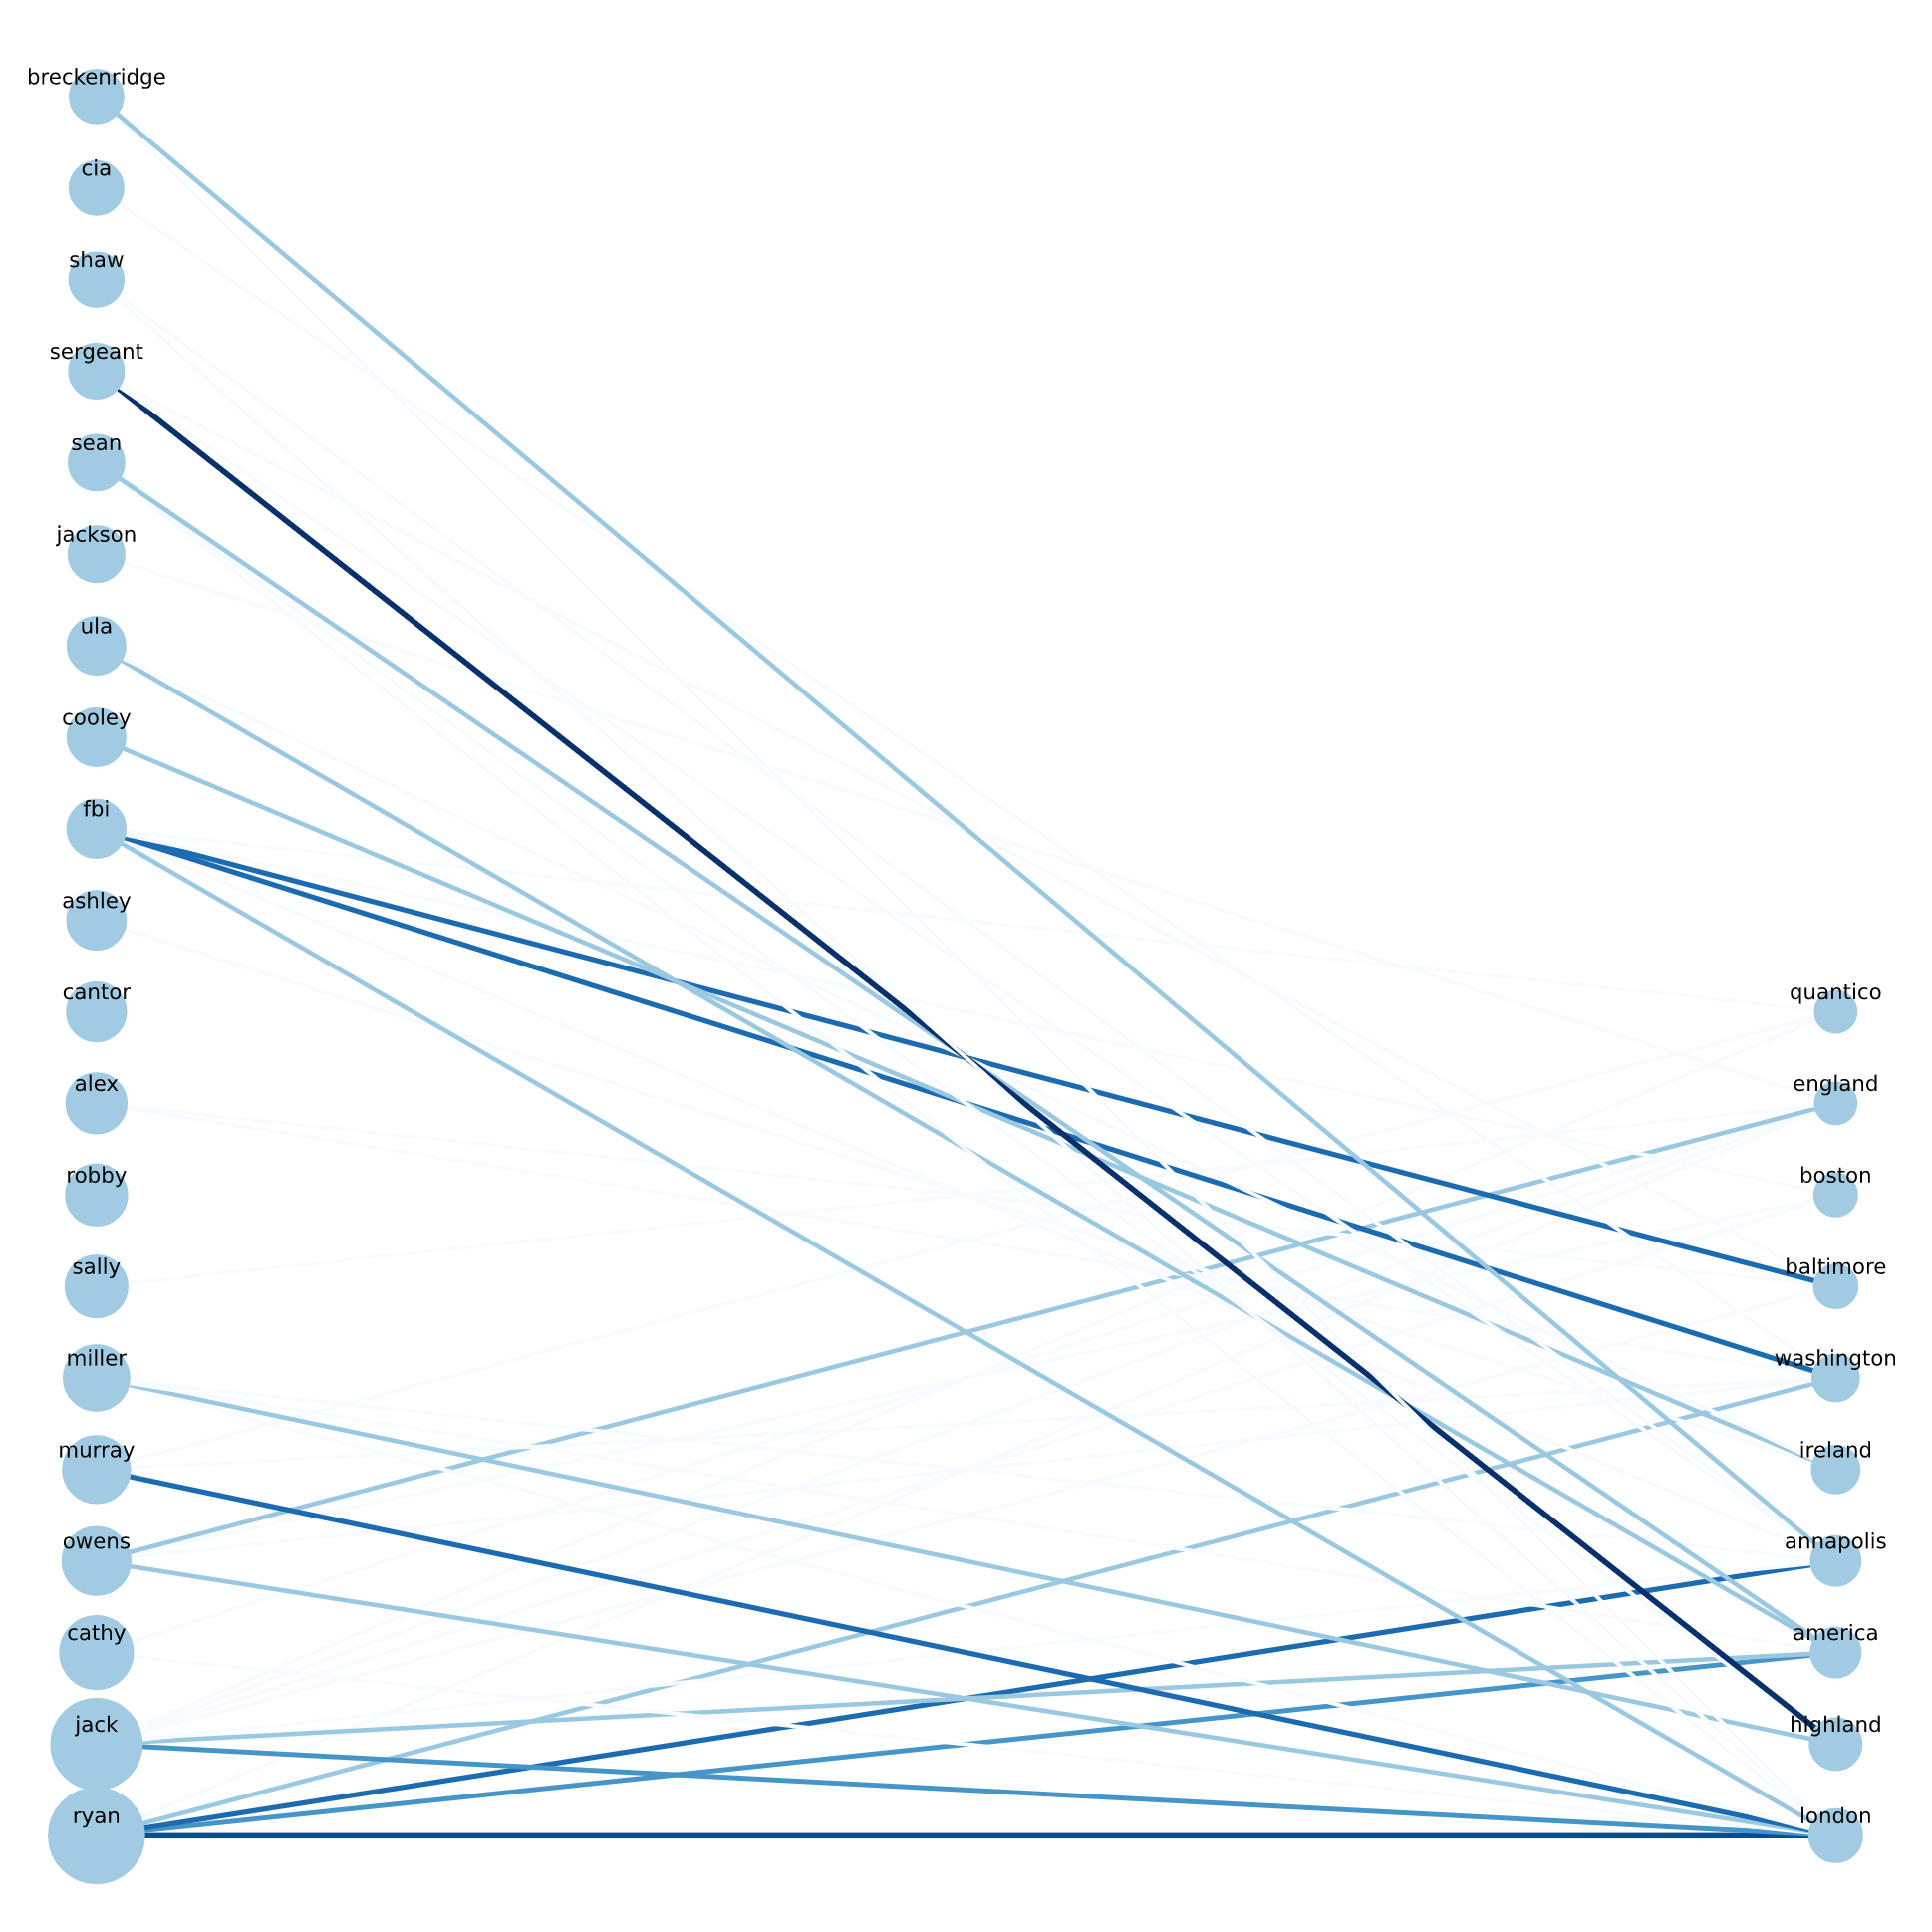
\includegraphics[width=10cm]{Tom Clancy - Patriot Games locations graph.png}
  \caption{Clancy Tom Patriot Game Locations Graph}
  \label{fig4}
\end{figure}

Either way, This graph shows pretty good results as a proof-of-concept for the idea, where the next stage would be comparing the model's results to tagged archaeology books and see the matching rate.

\section{Discussion}
The results shown here are primal, and further examination on a variety of novels is required to make any reliable point. There are still more directions that can be investigated and might lead to better and more reliable results, some of them are as follows.
\begin{itemize}
  \item Changing the co-occurrence method - We basically only looked at words that appeared in the same sentence as related words. Other scopes, such as a whole paragraph or even few following sentences might lead to more connections between certain characters and locations and better focus the main aspects of the book than the current method.
  \item Relations to references - The method used above only takes names into account and totally ignores more complicated references to them like "he", "she", "they" and so on... This causes a major lack of relational information as characters are usually referred to by those words and not by their name every time.
  \item Full names - As part of the solution, full names are split into first and last names and are counted separately, though it has it advantages, as it combines references to the same character even when it is mentioned differently, it also causes unwanted combination of characters (as few family members will all appear with the same last name), and also leads to split in the references of the same character (if the character sometimes referred to by its first name and sometimes by its last name). A technique to overcome this obstacle needs to be carefully examined to work properly.
\end{itemize}

\section{Code}
All the relevant code is available in a public github repository\cite{project2020}. This chapter will make an overview on the project files and folders.

\subsection{character\_network folder}
This folder contains a few key components in the solution. First is "character\_network\_iterative.py" which contains all the functions that needs to be run in the project, "Entire Process Notebook.ipynb" which is a notebook that runs the whole process on a book and creates the graph. The file contains 2 constants that needs to be replaced to run it on a different book, NOVEL\_FILE\_NAME with the path to the novel, and NOVEL\_NAME, for saving the results under the name of the novel. The folder also contains an output folder which contains the graphs created by the module.

\subsection{books folder}
This is basically a folder that contains the raw text of the books we want to use.
\subsection{reports folder}
This folder contains the report (this file) and the poster of the project.


\bibliographystyle{plain}
\bibliography{references}

\end{document}